\documentclass{article}
\usepackage[utf8]{inputenc}
\parskip = 0.75em
\parindent = 10mm
\def\baselinestretch{1}
\usepackage {float}
\usepackage{listings}
\usepackage{subcaption}
\usepackage[usenames]{color}
\usepackage[numbers,sort&compress]{natbib}
\usepackage{multirow, array}
\usepackage[spanish]{babel}
	\deactivatetilden
	\spanishdecimal{.}
	\addto\captionsspanish{\def\tablename{Tabla}}
	\addto\captionsspanish{\def\listtablename{\'Indice de tablas}}

\usepackage{amsmath,amsfonts,amssymb}
	\allowdisplaybreaks[4]
\usepackage{graphicx}
	\graphicspath{{Figuras/}}
\usepackage[clearempty,pagestyles]{titlesec}
\usepackage{anysize}

\def\baselinestretch{1.5}
\papersize{27.9cm}{21.5cm} 
\marginsize{2cm}{2cm}{1cm}{1cm}

\begin{document}


	\begin{center}
	\huge{\textbf{Tarea 8 Modelo de urnas}}\\
	
	\textsc{ \Large Susana Ruiz Nuñez}
	\end{center}


\section{Planteamiento del problema} 
En esta práctica \cite{satu} se tratan los fenómenos de coalescencia y fragmentación, donde partículas se unen para formar cúmulos y estos cúmulos se pueden volver a descomponer en fragmentos menores. Es de gran relevancia en muchos campos como por ejemplo en el filtrado de aguas residuales, donde solamente los cúmulos de suficiente tamaño serán capturadas por el filtro y hay que buscar formas para facilitar que crezcan los cúmulos de residuos para lograr su filtrado adecuado.

Se tiene para el problema inicial una cantidad \textit{n} total de  partículas y \textit{k} cúmulos existentes que siguen la distribución normal. Además se toma la mediana de los tamaños iniciales como el \textit{tamaño crítico c}: donde cúmulos menores a \textit{c}  solamente pueden pegarse uno al otro y quedarse como son, pero tamaños mayores a \textit{c} pueden además fragmentarse. La práctica consiste para diversas combinaciones de \textit{k, n} y el número de iteraciones \textit{t} hallar el porcentaje de partículas que se logra filtrar suponiendo que cúmulos con \textit{c} o más partículas son demasiado grandes para filtrar. 

\section{Metodología}
Se parte de un modelo base \cite{satu}, donde ya se tienen representados las funciones de rotura y unión del modelo. Primeramente se definen los tamaños de los valores con los que hay que hacer el experimento: n, k, t. Luego es necesario definir una función filtrar que con un mecanismo sencillo y basado en el valor de \textit{tamaño crítico c} elimine los valores que sobrepasen dicho tamaño. Este proyecto se realiza con Python 3.8 y a continuación se muestra el método utilizado. 
  

\begin{lstlisting}[language=Python]
	k = [100, 250, 500, 1000]
	n = [10000, 50000, 75000, 100000]
	t = [10, 25, 50, 100]
	# Eliminar los que sobrepasen el valor c : filtrado
	filtrados = []
	noFiltrados = []
	cumTotal = len(cumulos)
	for i in range(len(cumulos)):
		c = np.median(cumulos)
		if cumulos[i] > c:
			filtrados.append(cumulos[i])
		else:
			noFiltrados.append(cumulos[i])
	return ((len(filtrados) / cumTotal)*100)
\end{lstlisting}


\section{Resultados}
Los resultados obtenidos muestran una ligera variación en el porciento de filtrados cuando se cambian los valores de n, k y t. Vemos en la primera imagen el experimento se realiza para un mismo n y se varía el tamaño de los cúmulos. En la segunda imagen se hace para diferentes números de partículas y para el mismo número de cúmulos k.

\begin{figure}[H]
	\centering
	\begin{subfigure}[b]{0.45\linewidth}
		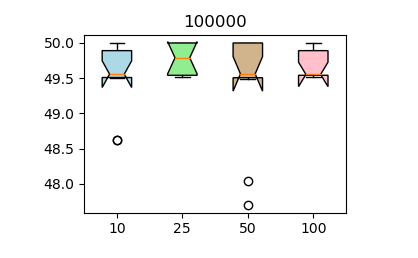
\includegraphics[width=\linewidth]{c100.png}
		\caption{Tamaño de los cúmulos 100.}
		\label{1}
	\end{subfigure}
		\begin{subfigure}[b]{0.45\linewidth}
		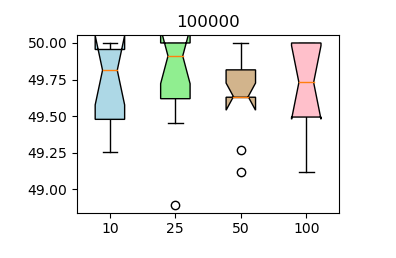
\includegraphics[width=\linewidth]{c250.png}
		\caption{Tamaño de los cúmulos 250.}
		\label{2}
	\end{subfigure}
		\begin{subfigure}[b]{0.45\linewidth}
			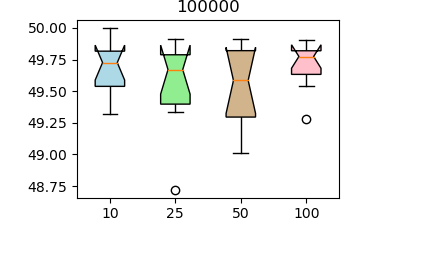
\includegraphics[width=\linewidth]{c500.png}
			\caption{Tamaño de los cúmulos 500.}
			\label{3}
	\end{subfigure}
		\begin{subfigure}[b]{0.45\linewidth}
				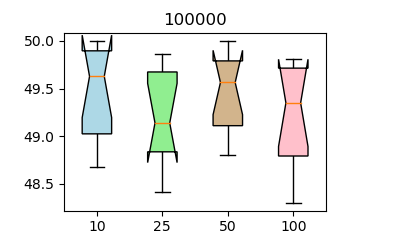
\includegraphics[width=\linewidth]{c1000.png}
				\caption{Tamaño de los cúmulos 1000.}
				\label{4}
	\end{subfigure}
	\caption{Porciento de total de filtrados para diferentes cúmulos k y para 100000 partículas(n).}  		
\end{figure}


\begin{figure}
\centering
	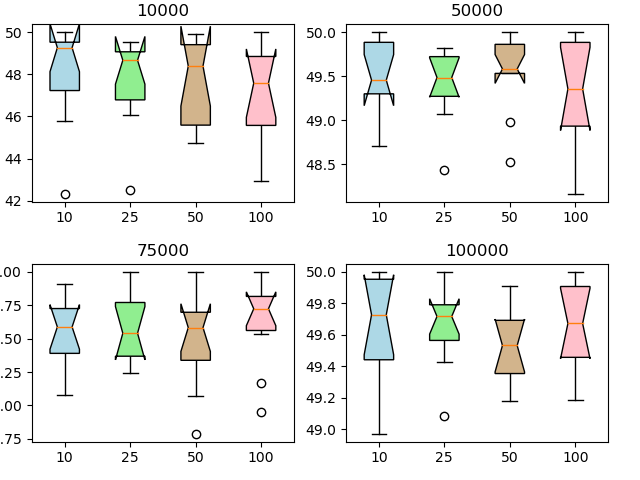
\includegraphics[width=\linewidth]{t8fig500.png}
	\caption{Porciento de filtrados para diferentes números de partículas n y para k = 500.}
	\label{1}		
\end{figure}
\section{Conclusiones}
Se concluye con los experimentos realizados que el aumento de los números de partículas, así como el tamaño de los cúmulos afecta ligeramente en los valores de filtrados que se obtienen. 

\bibliography{Tarea8}
\bibliographystyle{plainnat}
\end{document} 
